\documentclass{beamer}

\usepackage[utf8]{inputenc}
\usepackage{upgreek}
\usepackage{bm}
\usepackage{default}
\usepackage{algorithm,algorithmic}
\usepackage{amsmath,amssymb,amsfonts,graphicx,subfigure,tikz}
\beamertemplatenavigationsymbolsempty

\usetheme{Goettingen}

%\usetheme{Madrid}
\usecolortheme{seagull}





% 






%%%%%%%% tikz/pgf stuff: 
\newcommand{\defaultmarksize}{3pt}
\usepackage{tikz,pgfplots}
\usepackage{pgf}
%\usepackage{pgfmath}
\usepackage{pgffor}
%\pgfrealjobname{aof}
\usetikzlibrary{matrix}
\usetikzlibrary{calc}
\usetikzlibrary{arrows}
\usetikzlibrary{decorations.markings}
\usetikzlibrary{shapes,snakes}
\usetikzlibrary{calc}
\usetikzlibrary{plotmarks}
\usetikzlibrary{patterns}
\usepgflibrary[shapes.geometric]
\usetikzlibrary{snakes}
\usetikzlibrary{shapes.geometric}
\pgfplotsset{compat=newest}
%\pgfplotsset{plot coordinates/math parser=false}
\usepgflibrary{plothandlers} 



\newcommand{\RR}{\mathbb{R}}
\newcommand{\CC}{\mathbb{C}}
\newcommand{\diag}{\operatorname{diag}}

\newcommand{\mycite}[1]{$[$#1$]$}



\author[Giampaolo Mele]{Giampaolo Mele}
\title{The waveguide eigenvalue problem and Tensor infinite Arnoldi}
\institute{KTH Royal Institute of technology\\ Dept. Math, Numerical analysis group }
\date{27 August 2015 \\ \vspace{1cm} \small{Joint work with Elias  Jarlebring and Olof Runborg} \\ \vspace{1cm} \small{\textit{BIT Circus 2015 at Umeå University}} }



% \makeatletter
% \setbeamertemplate{sidebar canvas right}{}
% \setbeamertemplate{sidebar right}{%
%   \vspace*{\fill}
%   
\includegraphics[width=\beamer@sidebarwidth]{kth_logo.png}%
%   \vspace*{\fill}
% }
% \makeatother

\makeatletter
\addtobeamertemplate{sidebar right}{}{%
\vspace*{-10cm}

\includegraphics[width=\beamer@sidebarwidth]{kth_logo.png}%
\vspace*{\fill}
}
\makeatother



% redefinition of \insertverticalnavigation to get the desired highlighting for
% sections in the sidebar
\makeatletter
\def\insertverticalnavigation#1{%
  \vbox{%
    \def\sectionentry##1##2##3##4##5{%
      \ifnum##5=\c@part%
      \def\insertsectionhead{##2}%
      \def\insertsectionheadnumber{##1}%
      \def\insertpartheadnumber{##5}%
      \hbox{{%
        \usebeamerfont{section in sidebar}\usebeamercolor[fg]{section in sidebar}%
          \hyperlink{Navigation##3}{%
          \ifnum\c@section=##1%
            %\ifnum\c@subsection=0\relax% NEW
              {\usebeamertemplate{section in sidebar}}%
            %\else%% NEW
              \ifx\beamer@nav@css\beamer@hidetext%
                {\usebeamertemplate{section in sidebar}}%
              \else%
                {\usebeamertemplate{section in sidebar shaded}}%
              \fi%
            %\fi%% NEW
          \else
            {\usebeamertemplate{section in sidebar shaded}}%
          \fi}}}%
      \beamer@currentsubsection=0\relax\fi}%
    \def\slideentry##1##2##3##4##5##6{}%
    \def\beamer@subsectionentry##1##2##3##4##5{%
      \ifnum##1=\c@part%
      \def\insertpartheadnumber{##1}%
      \def\insertsectionheadnumber{##2}%
      \def\insertsubsectionheadnumber{##3}%
      \def\insertsubsectionhead{##5}%
       \beamer@tocifnothide{\ifnum\c@section=##2\ifnum\c@subsection=##3\beamer@nav@css\else\beamer@nav@oss\fi\else\beamer@nav@ooss\fi}%
      {\hbox{{%
        \usebeamerfont{subsection in sidebar}\usebeamercolor[fg]{subsection in sidebar}%
          \hyperlink{Navigation##4}{%
          \ifnum\c@section=##2%
            \ifnum\c@subsection=##3%
              \ifnum\c@subsubsection=0\relax%
                {\usebeamertemplate{subsection in sidebar}}%
              \else%
                {\usebeamertemplate{subsection in sidebar shaded}}%
              \fi%
            \else%
              {\usebeamertemplate{subsection in sidebar shaded}}%
            \fi%
          \else%
            {\usebeamertemplate{subsection in sidebar shaded}}%
          \fi}}}%
      }%
      \fi}%
    \def\beamer@subsubsectionentry##1##2##3##4##5##6{%
      \ifnum##1=\c@part%
      \def\insertpartheadnumber{##1}%
      \def\insertsectionheadnumber{##2}%
      \def\insertsubsectionheadnumber{##3}%
      \def\insertsubsubsectionheadnumber{##3}%
      \def\insertsubsubsectionhead{##6}%
      \beamer@tocifnothide{\ifnum\c@section=##2\ifnum\c@subsection=##3\beamer@nav@css\else\beamer@nav@oss\fi\else\beamer@nav@ooss\fi}%
      {\hbox{{%
        \usebeamerfont{subsubsection in sidebar}\usebeamercolor[fg]{subsubsection in sidebar}%
          \hyperlink{Navigation##5}{%
          \ifnum\c@section=##2%
            \ifnum\c@subsection=##3%
              \ifnum\c@subsubsection=##4%
                {\usebeamertemplate{subsubsection in sidebar}}%
              \else
                {\usebeamertemplate{subsubsection in sidebar shaded}}%
              \fi%
            \else%
              {\usebeamertemplate{subsubsection in sidebar shaded}}%
            \fi%
          \else%
            {\usebeamertemplate{subsubsection in sidebar shaded}}%
          \fi}}}%
      }%
      \fi}%
    %\beamer@currentsubsection=0\relax%
    \dohead%
  }%
}
\makeatother






% color definitions
\definecolor{konzeBlue}{RGB}{45,170,250}
\definecolor{konzeBlueLight}{RGB}{116,199,252}
\definecolor{mainTextColor}{RGB}{80,80,80}
\definecolor{titleTextColor}{RGB}{120,120,120}





% sidebar
\setbeamertemplate{sidebar canvas right}[vertical shading]%[top=Blue,bottom=Blue]
\setbeamercolor{author in sidebar}{fg=black}
\setbeamerfont{title in sidebar}{family=\normalfont,series=\bfseries}
\setbeamerfont{author in sidebar}{family=\normalfont,series=\bfseries,size={\fontsize{8}{12}}}
\setbeamercolor{section in sidebar}{fg=white}
\setbeamercolor{section in sidebar}{bg=konzeBlue}
\setbeamerfont{section in sidebar}{size=\tiny}
\setbeamerfont{section in sidebar}{series=\bfseries}
\setbeamercolor{subsection in sidebar}{fg=white}
\setbeamercolor{subsection in sidebar}{bg=konzeBlue}
\setbeamerfont{subsection in sidebar}{series=\tiny}




%\titlegraphic{
\includegraphics[width=2cm]{kth_logo.png}}

\begin{document}

\frame{\titlepage}

\begin{frame}
\frametitle{Outline}
\begin{itemize}
 \item WEP: Waveguide Eigenvalue Problem
 \item TIAR: Tensor infinite Arnoldi
 \item Specialization of TIAR to WEP and numerical simulations
\end{itemize}
\end{frame}

\newcommand\invisiblesection[1]{%
  \refstepcounter{section}%
  \addcontentsline{toc}{section}{\protect\numberline{\thesection}#1}%
  \sectionmark{#1}}
  

\section{ \ }
\section{ \ }
\section{ \ }
\section{ \ }
\section{ \ }

\newenvironment{specialframe}
{
    \begingroup
    \advance\textwidth2cm % see beamerthemeGoettingen.sty for the number
    \hsize\textwidth
    \columnwidth\textwidth
    \begin{frame}[plain]
}
{
    \end{frame}
    \endgroup
}




\section{WEP}

\begin{specialframe}{}
\begin{block}{\vspace*{-3ex}}
 \begin{center}
    \fontsize{30}{36}\selectfont WEP: the waveguide eigenvalue problem 
\end{center}
\end{block}
\end{specialframe}

\begin{frame}
\begin{block}{Helmholtz equation (single-periodic coefficients):}\vspace{-0.8cm}
\begin{eqnarray*}
  \Delta u(x,z)+\kappa(x,z)^2u(x,z)&=&0\;\; \textrm{when }\; (x,z)\in\RR\times\RR\\
  u(x,\cdot)&\rightarrow& 0\;\;\textrm{as }\; x\rightarrow\pm\infty
\end{eqnarray*}\vspace{-0.6cm}
\begin{itemize}
  \item $\kappa(x,z)$ periodic $z$-direction. 
  \item $\kappa(x,z)$ constant for $(x,z)\not\in[x_-,x_+]\times\RR$. 
\end{itemize}\vspace{-0.2cm}
\end{block}

\begin{center}
\scalebox{0.8}{%\tikzsetnextfilename{waveguidefig2} % name for the temporary 
\definecolor{cbebebf}{RGB}{200,200,200}%
\begin{tikzpicture}[remember picture, y=0.80pt,x=0.80pt,yscale=-0.25,xscale=0.25, inner sep=0pt, outer sep=0pt]
  %\path [use as bounding box,red] (300,112) rectangle (20.0000,292.36);
  \path[fill=cbebebf,line join=miter,line cap=butt,even odd rule,line
    width=0.800pt,rounded corners=0.0000cm] (70.0000,112.3622) rectangle
    (680.0000,292.3622);
  \node at (360,60) {$\vdots$};
  \node at (0.0000,180) (myref) {};
%  \path[draw=black,line join=miter,line cap=butt,line width=0.800pt]
%    (650.0000,112.3622) .. controls (100.0000,112.3622) and (100.0000,112.3622) ..
%    (100.0000,112.3622);
%  \path[draw=black,line join=miter,line cap=butt,line width=0.800pt]
%    (650.5000,291.8622) .. controls (100.5000,291.8622) and (100.5000,291.8622) ..
%    (100.5000,291.8622);
  \path[draw=black,line join=miter,line cap=butt,line width=1.800pt]
    (300.0000,112.3622) -- (300.0000,292.3622) -- (300.0000,292.3622);
  \path[draw=black,line join=miter,line cap=butt,line width=1.800pt]
    (380.0000,112.3622) -- (380.0000,232.3622) -- (420.0000,232.3622) --
    (420.0000,292.3622) -- (420.0000,292.3622);
  \path[fill=black] (255.56859,334.04221) node (text3878) {\phantom{$\;\;\;\partial\Omega_-$}};
  \path[fill=black] (440.42651,334.04221) node[right] (text3882) {\phantom{$\partial\Omega_+$   }};
  \node at (0,690) {};
\end{tikzpicture}%
\begin{tikzpicture}[remember picture, y=0.80pt,x=0.80pt,yscale=-0.25,overlay, shift={(myref.north)}, xscale=0.25, inner sep=0pt, outer sep=0pt]
  \path[fill=cbebebf,line join=miter,line cap=butt,even odd rule,line
    width=0.800pt,rounded corners=0.0000cm] (70.0000,112.3622) rectangle
    (680.0000,292.3622);
  \node at (0.0000,180) (myref2) {};
%  \path[draw=black,line join=miter,line cap=butt,line width=0.800pt]
%    (650.0000,112.3622) .. controls (100.0000,112.3622) and (100.0000,112.3622) ..
%    (100.0000,112.3622);
%  \path[draw=black,line join=miter,line cap=butt,line width=0.800pt]
%    (650.5000,291.8622) .. controls (100.5000,291.8622) and (100.5000,291.8622) ..
%    (100.5000,291.8622);
  \path[draw=black,line join=miter,line cap=butt,line width=1.800pt]
   (300.0000,112.3622) -- (300.0000,292.3622) -- (300.0000,292.3622);
  \path[draw=black,line join=miter,line cap=butt,line width=1.800pt]
    (425,112.3622) --  (380.0000,112.3622) -- (380.0000,232.3622) -- (420.0000,232.3622) --
    (420.0000,292.3622) -- (420.0000,292.3622);
\end{tikzpicture}%
\begin{tikzpicture}[remember picture, y=0.80pt,x=0.80pt,yscale=-0.25,overlay, shift={(myref2.north)}, xscale=0.25, inner sep=0pt, outer sep=0pt]
  \path[fill=cbebebf,line join=miter,line cap=butt,even odd rule,line
    width=0.800pt,rounded corners=0.0000cm] (70.0000,112.3622) rectangle
    (680.0000,292.3622);
  \node at (0.0000,180) (myref3) {};
%  \path[draw=black,line join=miter,line cap=butt,line width=0.800pt]
%    (650.0000,112.3622) .. controls (100.0000,112.3622) and (100.0000,112.3622) ..
%    (100.0000,112.3622);
%  \path[draw=black,line join=miter,line cap=butt,line width=0.800pt]
%    (650.5000,291.8622) .. controls (100.5000,291.8622) and (100.5000,291.8622) ..
%    (100.5000,291.8622);
  \path[draw=black,line join=miter,line cap=butt,line width=1.800pt]
   (300.0000,112.3622) -- (300.0000,292.3622) -- (300.0000,292.3622);
  \path[draw=black,line join=miter,line cap=butt,line width=1.800pt]
    (425,112.3622) --  (380.0000,112.3622) -- (380.0000,232.3622) -- (420.0000,232.3622) --
    (420.0000,292.3622) -- (420.0000,292.3622);
  \path[<->,draw=black,line width=1pt]
    (100.0000,150) -- node[midway,left] {$z$\;\;} (100.0000,240) -- node[midway,below]{$\phantom{\Sigma^\Sigma}x\phantom{\Sigma^\Sigma}$} (200,240);
  \node at (360,320) {$\vdots$};
\end{tikzpicture}%
}%
\end{center}


\underline{Some related computational works}:
\mycite{Tausch, Butler '02}, \mycite{Engstr\"om, Hafner, Schmidt '09, Engstr\"om '10}, \mycite{Schmidt, Hiptmair '13}, \mycite{Spence, Poulton '05},  \mycite{Cox, Stevens '99}, $\ldots$ 


\end{frame}


\begin{frame}
We look for normal modes (Bloch solutions)
\begin{eqnarray*}
  u(x,z)&=&e^{\lambda z}v(x,z) \\
  v(x,z)&=&v(x,z+1)\;\;\;\;\;\Rightarrow
\end{eqnarray*}
\vspace{-0.8cm}
\begin{block}{Periodic PDE-eigenvalue problem on a strip}
Find $v\in\mathcal{C}^1(\RR\times[0,1],\RR)$ and $\lambda$ such that:
\begin{eqnarray*}
\Delta v+2\lambda v_z+(\lambda^2+\kappa(x,z)^2)v&=&0\\
  v(\cdot,z)&\rightarrow& 0\;\;\textrm{as }\; x\rightarrow\pm\infty\\
  v(x,z)&=&v(x,z+1)
\end{eqnarray*}
%\hfill See preprint for 
\end{block}
\begin{center}
\scalebox{0.4}{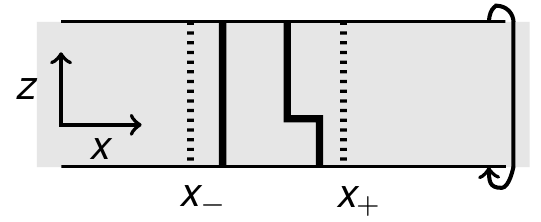
\includegraphics{wep_fig.png}}%
\end{center}
Solutions of most interest: $\lambda\in\CC_-$ close to imaginary axis.
\end{frame}

\begin{frame}

\begin{block}{DtN (Dirichlet to Neumann) equivalence}
 Under generic conditions, equivalent in a weak sense
\vspace{-0.1cm}\small \begin{eqnarray*} \hspace{-0cm}
\Delta v+2\lambda v_z+(\lambda^2+\kappa(x,z)^2)v&=&0,
\;\; (x,z)\in[x_-,x_+]\times [0,1]\\
  v(x,z)&=&v(x,z+1)\\
  v_x(x_-,\cdot)&=&\mathcal{T}_{-,\lambda}(v(x_-,\cdot))\\
  v_x(x_+,\cdot)&=&\mathcal{T}_{+,\lambda}(v(x_+,\cdot))
\end{eqnarray*}
$\mathcal{T}_{\pm,\lambda}(\cdot)$ has nonlinear dependence in $\lambda$.
\end{block}

\begin{block}{Discretized problem}
 A particular type of FEM discretization leads to 
\[
  M(\lambda)v=
  \begin{pmatrix}
    Q(\lambda) & C_1 (\lambda)\\
    C_2^T & R^HP(\lambda)R
  \end{pmatrix} v = 0
\]
\end{block}
$P(\lambda)$ nonlinear and non polynomial in $\lambda$. 
\end{frame}

\section{TIAR}




\begin{frame}
\begin{block}{The nonlinear eigenvalue problem}
Find $\lambda\in\CC$, $v\neq 0$ such that
\begin{equation*}
  M(\lambda)v=0
\end{equation*}
where $M$ analytic in a disk $\Omega\subset\CC$. \\
\end{block}
\begin{block}{Selection of interesting works}
\small  \mycite{Ruhe '73}, \mycite{Mehrmann, Voss '04},
\mycite{Lancaster '02}, 
\mycite{Tisseur,~et~al.~'01}, \mycite{Voss '05}, \mycite{Unger~'50}, \mycite{Mackey, et al. '09}, 
\mycite{Kressner '09}, 
\mycite{Bai, et al. '05}, \mycite{Meerbergen '09}, \mycite{Breda, et al. '06},
\mycite{Betcke, et al. '04, '10}, 
\mycite{Asakura, et a. '10}, 
\mycite{Beyn '12}, \mycite{Szyld, Xue '13},
\mycite{Hochstenbach,~et al.~'08}, \mycite{Neumaier '85},
\mycite{Gohberg, et al. '82}, \mycite{Effenberger '13},
\mycite{Van Beeumen, et al '15}
\ldots
%Framework for automized solving  \eqref{eq:nlevp} in a reliable efficient way.
\end{block}
\end{frame}







\begin{specialframe}{}
\begin{block}{\vspace*{-3ex}}
 \begin{center}
    \fontsize{30}{36}\selectfont TIAR: tensor infinite Arnoldi
\end{center}
\end{block}
\end{specialframe}







\begin{frame}
\begin{block}{Properties / features of infinite Arnoldi method}
\begin{itemize}
  \item Equivalent to Arnoldi's method on a companion matrix, \\ for any truncation parameter $N$ with $N>k$
  \item Equivalent to Arnoldi's method on an operator $\mathcal{B}$
  \item Convergence theory (?)   
  %\item Eigenvalue equivalence: $\{1/\lambda_i \}_{i=0}^\infty\backslash\{0\}=\sigma(\mathcal{B})\backslash\{0\}$
  \item Requires adaption of computation of $y_0$. For Taylor version: 
\[
y_0=M(\hat{\lambda})^{-1}(M'(\hat{\lambda})x_1+\cdots+M^{(k)}(\hat{\lambda})x_k)
\]\vspace{-0.6cm}
 \item Complexity of orthogonalization at step $k$: $O(k^2n)$
\end{itemize}
\end{block}
%\begin{block}
{Described in:}
\mycite{Jarlebring,~et~al.~'11, '12, '15} 
%Framework for automized solving  \eqref{eq:nlevp} in a reliable efficient way.
%\end{block}
\end{frame}


\begin{frame}
%{Tensor ``resolution'' to $\mathcal{O}(m^3n)$ complexity.}
\vspace{-0.1cm}
\begin{block}{Observation: The basis matrix has a structure}
\begin{center}
\scalebox{0.5}{\tikzset{
  big arrow/.style={
    decoration={markings,mark=at position 1 with {\arrow[scale=1.5,#1]{>}}},
    postaction={decorate},
    shorten >=0.4pt},
  big arrow/.default=black}

\begin{tikzpicture}[y=0.80pt,x=0.80pt]
  \matrix (m) [matrix of math nodes,row sep=1em,column sep=2em,minimum width=2em, 
%  \matrix (m) [matrix of math nodes,row sep=0em,column sep=0em,minimum width=2em, 
%style={nodes={inner sep=0,minimum height=2cm, draw}},
style={nodes={inner sep=0,circle, draw}},
%row 1/.style={nodes={inner sep=0,draw,solid}},
column 6/.style={nodes={inner sep=0,draw,solid}},
column 8/.style={nodes={inner sep=0,draw,solid}},
]
  {
     v_{00}& v_{01} & v_{02} & v_{03} &  \\ 
                & v_{11} & v_{12} & v_{13}  & \\ 
                &            & v_{22} & v_{23}      & \\ 
                &            &                & v_{33}      &  \\ 
               &            &                &                     & \\ };
%  \node (aa) at (m-2-2) { };
%  \draw (m-1-1) -- (m-1-2);
  %\draw[dashed] (m-1-1) -- (m-2-2);
  
  %\draw (m-1-2) -- (m-1-3);
 % \draw[dashed] (m-1-2) -- (m-2-3);
 % \draw[dashed] (m-2-2) -- (m-3-3);
 % \draw[dashed](m-2-2) -- (m-2-3);
 % \draw (m-2-2) -- (m-1-3);
 
 % \draw (m-1-3) -- (m-1-4);
 % \draw[dashed] (m-1-3) -- (m-2-4);
 % \draw[dashed] (m-2-3) -- (m-3-4);
 % \draw[dashed] (m-2-3) -- (m-2-4);
 % \draw[dashed] (m-3-3) -- (m-4-4);
 % \draw[dashed] (m-3-3) -- (m-3-4);
 %  \draw (m-2-3) -- (m-1-4);
 % \draw (m-3-3) -- (m-1-4);
\pause
\matrix (y) [
matrix of math nodes,
row sep=1em,column sep=2em,minimum width=2em,anchor=north west,
style={nodes={inner sep=0,circle,draw}},
] at ($(m.north east)+(0.5,0)$) {
y_0 &\\ 
 y_1 \\ 
 y_2 \\ 
 y_3 \\ 
 y_4 \\ 
};
%% y-computation

   \draw[dashed,big arrow] (m-1-4) -- (y-2-1);
   \draw[dashed,big arrow] (m-2-4) -- (y-3-1);
   \draw[dashed,big arrow] (m-3-4) -- (y-4-1);
   \draw[dashed,big arrow] (m-4-4) -- (y-5-1);
   \draw[big arrow] (y-2-1) to [bend right] (y-1-1);
   \draw[big arrow] (y-3-1) to [bend right] (y-1-1);
   \draw[big arrow] (y-4-1) to [bend right] (y-1-1);
   \draw[big arrow] (y-5-1) to [bend right] (y-1-1);
 
\pause
\matrix (vp) [
matrix of math nodes,
row sep=1em,column sep=2em,minimum width=2em,anchor=north west,
style={nodes={inner sep=0,circle,draw}},
] at ($(y.north east)+(0.5,0)$) {
v_{04} \\ 
 v_{14} \\ 
 v_{24} \\ 
 v_{34} \\ 
 v_{44} \\ 
};
 
%% v computation
  \draw[dashed,big arrow] (m-1-1) to [bend left=20] (vp-1-1);
  \draw[dashed,big arrow] (m-1-2) to [bend left=20] (vp-1-1);
  \draw[dashed,big arrow] (m-1-3) to [bend left=20] (vp-1-1);
  \draw[dashed,big arrow] (m-1-4) to [bend left=20] (vp-1-1);
  \draw[dashed,big arrow] (y-1-1) to [bend left=20] (vp-1-1);

  \draw[dashed,big arrow] (m-2-2) to [bend left=20] (vp-2-1);
  \draw[dashed,big arrow] (m-2-3) to [bend left=20] (vp-2-1);
  \draw[dashed,big arrow] (m-2-4) to [bend left=20] (vp-2-1);
  \draw[dashed,big arrow] (y-2-1) to [bend left=20] (vp-2-1);

  \draw[dashed,big arrow] (m-3-3) to [bend left=20] (vp-3-1);
  \draw[dashed,big arrow] (m-3-4) to [bend left=20] (vp-3-1);
  \draw[dashed,big arrow] (y-3-1) to [bend left=20] (vp-3-1);

  \draw[dashed,big arrow] (m-4-4) to [bend left=20] (vp-4-1);
  \draw[dashed,big arrow] (y-4-1) to [bend left=20] (vp-4-1);
%  \draw [-to,shorten >=-1pt,dashed,->,big arrow] (y-5-1) to [bend left=20] (vp-5-1);
  \draw[dashed,big arrow] (y-5-1) to [bend left=20] (vp-5-1);


\end{tikzpicture}
} \vspace{-0.5cm}
\end{center}
\end{block}\vspace{-0.1cm}
\begin{theorem}[Implicit representation of the basis matrix \mycite{Jarlebring, M., Runborg '15}]
There exists  $Z=[z_1,\ldots,z_k]\in\CC^{n\times k}$
and tensor $[a_{i,j,\ell}]_{i,j,\ell=1}^k$,
such 
that the blocks in the basis matrix generated by 
$k$ steps of  infinite 
Arnoldi method can factorized as
\[
  q_{i,j}=\sum_{\ell=1}^k a_{i,j,k} z_k.
\]
\end{theorem}
\end{frame}

\begin{frame}
\begin{block}{Key ideas of TIAR}
  \begin{itemize}
    \item Rephrase IAR using implicit representation
      of basis matrix as a $Z\in\CC^{n\times k}$ and $[a_{i,j,\ell}]_{i,j,\ell=1}^k$.
    \item Maintain orthogonality of $Z$ for numerical stability\
    %\item Equivalent to IAR (under generic conditions) and involves less memory $\mathcal{O}(nm^2)$ vs. $\mathcal{O}(nm)$.
  \end{itemize}
\end{block}\
\begin{block}{TIAR vs IAR}
 \begin{itemize}
  \item TIAR involves less memory $\mathcal{O}(nm^2)$ vs. $\mathcal{O}(nm)$, 	\\
  \item Complexity for $m$ steps: $\mathcal{O}(nm^3)$ for both,			\\
  \item TIAR involves less data and is much faster
	  due to modern CPU-caching issues
 \end{itemize}
\end{block}\
{Other literature with compact representations}
  \begin{itemize}
    \item TOAR: \mycite{Zhang, Su, '13}, \mycite{Kressner, Roman '14}
    \item CORK: \mycite{V. Beeumen, et al '15}
  \end{itemize}
\end{frame}


% \begin{frame}
% \begin{block}{Complexity considerations}
%   Memory: $m$ steps of IAR vs TIAR:
%   \begin{itemize}
%     \item IAR: $\mathcal{O}(nm^2)$
%     \item TIAR: $\mathcal{O}(nm)$
%   \end{itemize}\
%   Computation time IAR and TIAR at step $k$: 
%   \begin{itemize}
%     \item[(i)] Dominating cost IAR: $h=Q_k^Tv$, $Q_k\in\RR^{nk\times k}$, $v\in\RR^{nk}$: 
% \[\mathcal{O}(nk^2)
% \]\
%     \item[(ii)] Dominating cost TIAR: $Y=Z_kA$, $Z_k\in\RR^{n\times k}$, $A\in\RR^{k\times k}$: 
% \[\mathcal{O}(nk^2)
% \]
%   \end{itemize}\
% In practice: (ii) involves less data and extremely much faster
% due to modern CPU-caching issues. 
% \end{block}
%\end{frame}

\section{Combination}
\begin{specialframe}{}
\begin{block}{\vspace*{-3ex}}
 \begin{center}
    \fontsize{30}{36}\selectfont Specialization of TIAR to WEP and numerical simulations
\end{center}
\end{block}
\end{specialframe}


\begin{frame}{}%{Cayley transformation}
%One derivation of IAR is via Taylor expansion. %$\Rightarrow$~\\
%Justification of convergence only guaranteed in convergence
%disk. ~\\
Recall WEP: \[
  M(\lambda)=
  \begin{pmatrix}
    Q(\lambda) 	& C_1(\lambda)	\\
    C_2^T 	& R^HP(\lambda)R
  \end{pmatrix}\
\]
 and $Q(\lambda)=A_0+A_1\lambda+A_2\lambda^2$ and~$C_1(\lambda)=C_{1,0}+C_{1,1}\lambda+C_{1,2}\lambda^2$ 
 %, $R$ corresponds to FFT \ and
 \[
   P(\lambda)=
 \diag(s_{-,-p}(\lambda),\ldots,s_{-,p}(\lambda),
 s_{+,-p}(\lambda),\ldots,s_{+,p}(\lambda))
 \]
where 
\[
s_{\pm,k}(\lambda)=\rho_k \sqrt{((\lambda+2i\pi k)+i\kappa_\pm)((\lambda+2i\pi k)-i\kappa_\pm)}.
\]\
{\bf Bad news:} $\mathcal{O}(\sqrt{n})$ branch-point  singularities~\\
{\bf Good news:} All singularities are on $i\RR$~\\\
%\vspace{-1cm}
\begin{block}{Solution}
Cayley transformation brings all singularities to unit circle. ~\\
Apply algorithm to Cayley transformed problem.
\end{block}
\end{frame}

\begin{frame}
In order to implement IAR or TIAR: We need an efficient way to compute
\[
y_0=M(0)^{-1}(M'(0)x_1+\cdots+M^{(k)}(0)x_k)
\]
\begin{block}{Compute by exploiting structure}
\begin{itemize}
  \item Derivatives of $\sqrt{a\lambda^2+b\lambda+c}$ after Cayley transformation computable with Gegenbauer polynomials (inspired by \mycite{Tausch, Butler 02'})
  \item Use FFT-for dense (2,2)-block
  \item Higher order derivatives have $\mathcal{O}(\sqrt{n})$ non-zero
elements (reduces dominant $\mathcal{O}(n)$-term to $\mathcal{O}(\sqrt{n})$)
  \item Use Schur complement and LU-factorization of $(1,1)$-block
\end{itemize}
\end{block}
\end{frame}

\section{Simulations}
\begin{frame}
%$\ldots$ back to the WEP
Simulations for a (more difficult) variant of the waveguide in \mycite{Tausch,~Butler~'02}
\begin{center}%
\scalebox{0.4}{
\includegraphics{waveguide_geometry.pdf}}%
\end{center}
One of the eigenfunctions of interest
\scalebox{0.55}{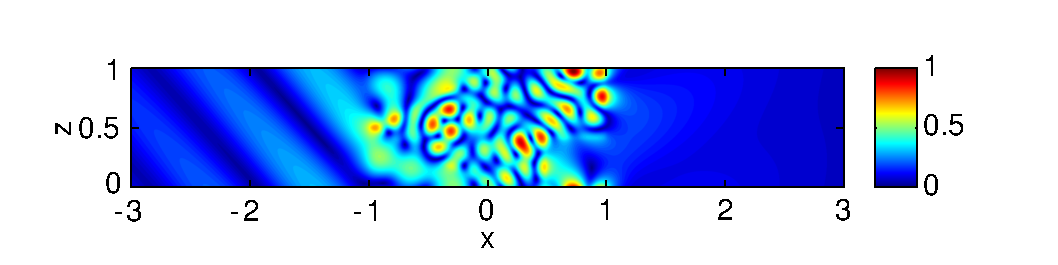
\includegraphics{eigenfunction.pdf}}\\

\hfill Largest problem with our approach: $n\approx 10^7$.
\end{frame}



\begin{frame}[plain]%{Simulations - TIAR and waveguide eigenvalue problem}
\scalebox{0.55}{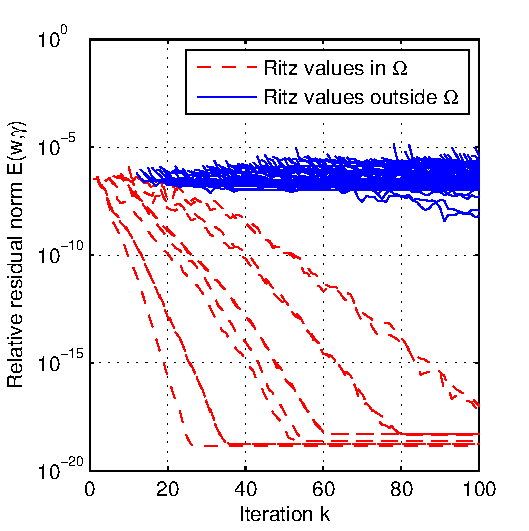
\includegraphics{error_hist.pdf}}%
\scalebox{0.30}{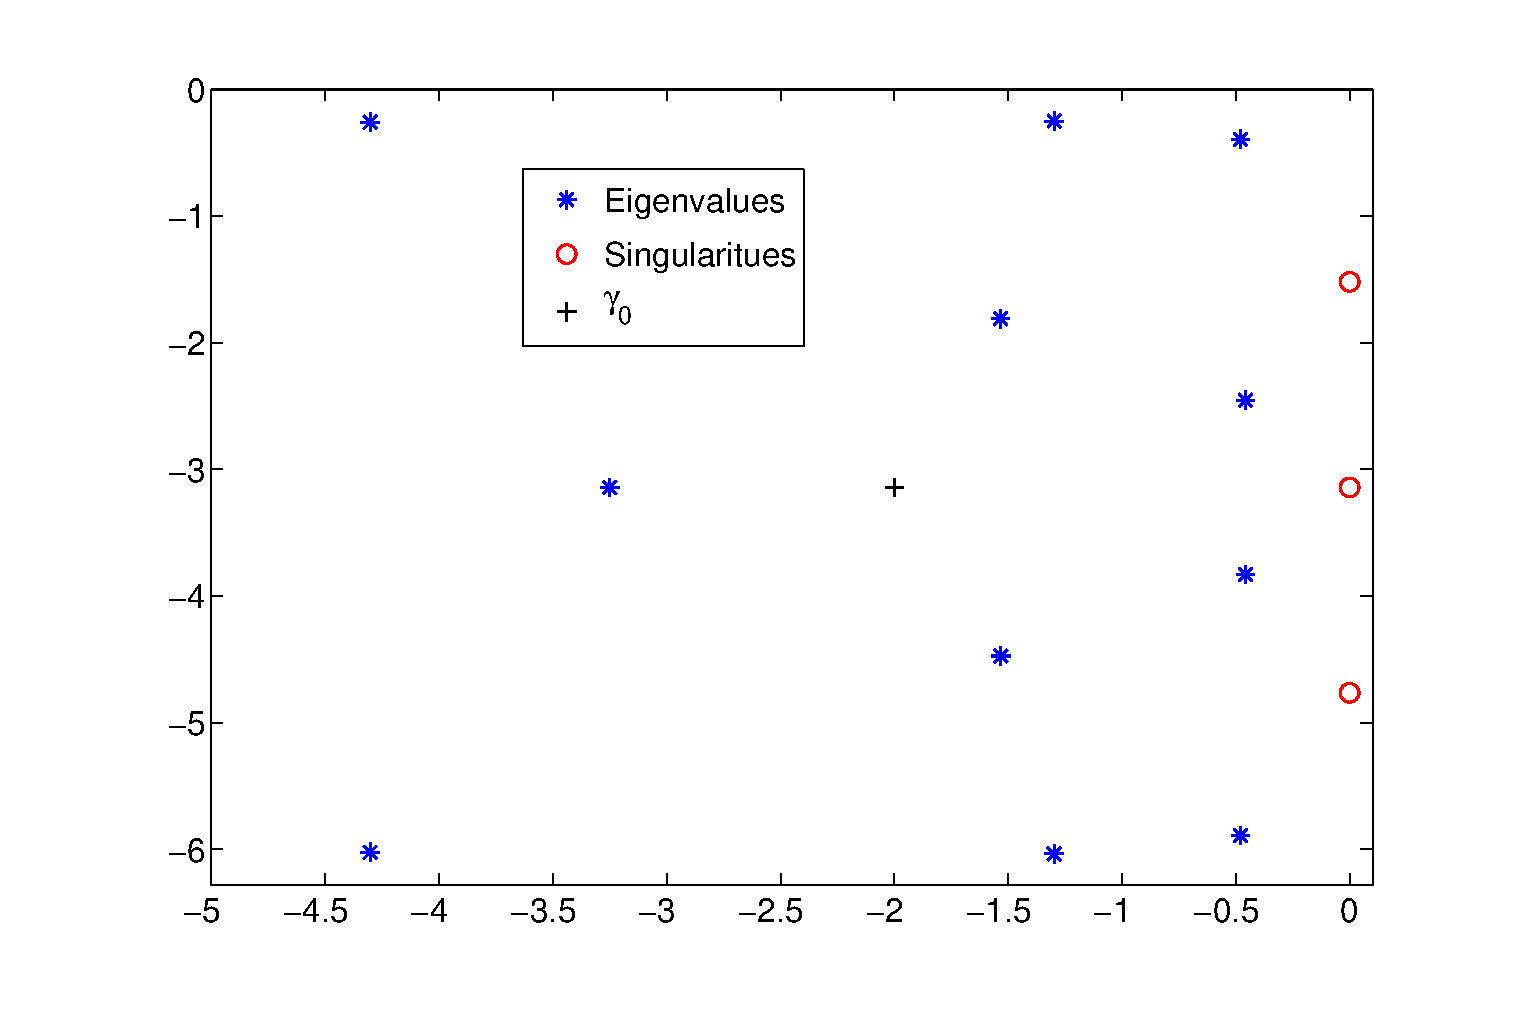
\includegraphics{eigenvalues_challenging_waveguide2.eps}}%

\vspace{-0.5cm}
 \begin{center}
   \resizebox{12cm}{!} {
    \begin{tabular}{c|c|c|c|c|c|c|}
     \cline{4-7}
		\multicolumn{3}{c}{}		&	 \multicolumn{2}{|c|}{CPU time } 			&	\multicolumn{2}{|c|}{storage of $Q_m$} 		\\
\hline
\multicolumn{1}{|c|}{$n$}		&	$n_x$	&	$n_z$	&	  IAR				&				WTIAR&	 		IAR 		&	 TIAR				\\
\hline
\multicolumn{1}{|c|}{462}		&	20	&	21	& 	 8.35 secs			&		2.58 secs		&		35.24 MB	&	7.98 MB				\\
\hline
\multicolumn{1}{|c|}{1,722}		&	40	&	41	& 	 28.90 secs			&		2.83 secs		&		131.38 MB	&	8.94 MB				\\
\hline
\multicolumn{1}{|c|}{6,642}		&	80	&	81	& 	1 min and 59 secs		&		4.81 secs		&		506.74 MB	&	12.70 MB			\\
\hline
\multicolumn{1}{|c|}{26,082}		&	160	&	161	& 	8 mins and 13.37 secs		&		13.9 secs		&		1.94 GB		&	27.52 MB			\\
\hline
\multicolumn{1}{|c|}{103,362}		&	320	&	321	& 	out of memory			&		45.50 secs		&		out of memory	&	86.48 MB			\\
\hline
\multicolumn{1}{|c|}{411,522}		&	640	&	641	& 	out of memory			&		3 mins and 30.29 secs	&		out of memory	&	321.60 MB			\\
\hline
\multicolumn{1}{|c|}{1,642,242}		&	1280	&	1281	& 	out of memory			&		15 mins and 20.61 secs	&		out of memory	&	1.23 GB				\\
\hline
\end{tabular}
}
 \end{center}
% \caption{CPU time and estimated memory required to perform $m=100$ iterations of IAR and WTIAR. The memory requirements
%for the storage of the basis is the same TIAR and WTIAR.}
 %\label{tbl:cputime_and_memory_IARvsTIAR}
{\small 
Using different computer: 
$n=9,009,002$, several hours CPU-time.}
%figure with profiling aspects

\end{frame}


\section{Conclusions}
\begin{frame}
 \begin{center}
    \fontsize{20}{24}\selectfont CONCLUSIONS
\end{center}

\begin{block}{New contributions}
  \begin{itemize}
    \item A structured discretization of a waveguide eigenvalue problem (WEP)
    \item A new algorithm: TIAR
    \item Specialization of TIAR to WEP
  \end{itemize}
\end{block}
\medskip
Online material:
\begin{itemize}
  \item Preprint: \\\url{http://arxiv.org/abs/1503.02096}
  \item Software: \url{http://www.math.kth.se/~gmele/waveguide}
\end{itemize}
\end{frame}


% \begin{frame}
% In order to implement IAR or TIAR: We need an efficient way to compute
% \[
% y_0=M(0)^{-1}(M'(0)x_1+\cdots+M^{(k)}(0)x_k)
% \]\
% \begin{block}{Compute by exploiting structure}
% \begin{itemize}
%   \item Derivatives of $\sqrt{a\lambda^2+b\lambda+c}$ after Cayley transformation computable with Gegenbauer polynomials (inspired by \mycite{Tausch, Butler 02'})
%   \item Use FFT-for dense (2,2)-block
%   \item Higher order derivatives have $\mathcal{O}(\sqrt{n})$ non-zero
% elements (reduces dominant $\mathcal{O}(n)$-term to $\mathcal{O}(\sqrt{n})$)
%   \item Use Schur complement and LU-factorization of $(1,1)$-block
% \end{itemize}
% \end{block}
% \end{frame}
% 







% \begin{frame}
% 
% \begin{block}{Discrete problem [WEP]}
% \[
%   M(\lambda)v=
%   \begin{pmatrix}
%     Q(\lambda) & C_1 (\lambda)\\
%     C_2^T & R^HP(\lambda)R
%   \end{pmatrix} v = 0
% \]
% \end{block}
% 
% \setbeamertemplate{itemize items}[ball]
% \begin{itemize}
%  \item solutions of interest: $\lambda \in \CC_-$ close to imaginary axis
%  \item $Q(\lambda)	=A_0+\lambda A_1+\lambda^2 A_2$ \hfill $A_i$ sparse
%  \item $C_1(\lambda)	=C_{1,0}+\lambda C_{1,1}+\lambda^2 C_{1,2}$ \hfill $C_{1,i}$ sparse
%  \item $C_2^T$ sparse
%  \item $Rx$ computed with FFT
%  \item $P(\lambda)$ diagonal matrix: 
%  \begin{itemize}
%   \item[-] nonlinear dependence on $\lambda$,
%   \item[-] derivatives available,
%   \item[-] singularities in $i \RR$ (close to solutions of interest!).
%  \end{itemize}
% \end{itemize}
%  After a Cayley transformation on $M(\lambda)$: 
%  \begin{itemize}
%   \item solutions of interest $|\lambda|<1$
%   \item $| \mbox{singularities} |=1$
%  \end{itemize}



%\end{frame}


% \begin{frame}{Absorbing boundary conditions}
% %\begin{overlayarea}{1.1\textwidth}{1.1\textheight}
% \begin{block}{DtN equivalence}
% \small Under generic conditions, equivalent in a weak sense
% \begin{itemize}
%   \item[(i)] A solution to PDE-eigenvalue problem on strip $u$. 
% \item[(ii)] A solution to 
% %\begin{minipage}{0.7\textwidth}\small
% \vspace{-0.1cm}\small \begin{eqnarray*} \hspace{-1cm}
% \Delta v+2\lambda v_z+(\lambda^2+\kappa(x,z)^2)v&=&0,
% \;\; (x,z)\in[x_-,x_+]\times [0,1]\\
%   v(x,z)&=&v(x,z+1)\\
%   v_x(x_-,\cdot)&=&\mathcal{T}_{-,\lambda}(v(x_-,\cdot))\\
%   v_x(x_+,\cdot)&=&\mathcal{T}_{+,\lambda}(v(x_+,\cdot))\\
% \end{eqnarray*}
% %\end{minipage}
% \end{itemize}\vspace{-0.9cm}
% \hfill For formalized weak-sense formulation in preprint
% \end{block}
% \small Dirichlet-to-Neumann maps in Fourier space:
% \[ 
% \mathcal{T}_{\pm,\lambda}
% \left(\sum_{k=-\infty}^\infty a_{\pm,k}e^{i2\pi kz}\right)
% =
% \sum_{k=-\infty}^\infty s_{\pm,k}(\lambda)a_{\pm,k}e^{i2\pi kz}.
% \]
% where $s_{\pm,k}=\rho_k \sqrt{((\lambda+2i\pi k)+i\kappa_\pm)((\lambda+2i\pi k)-i\kappa_\pm)}$ \\ 
% \begin{center}
% %\input{waveguidefig.tex}~\\
% %\includegraphics{schematic_interior.pdf}
% %\fbox{* figure with only rectangle *\phantom{\huge $X_\Sigma^\Sigma$}}
% %\fbox{* figure with only rectangle *\phantom{\huge $X_\Sigma^\Sigma$}}
% \end{center}
% %\end{overlayarea}
% \end{frame}




\end{document}

